%---------------------------------
% Preamble
%---------------------------------
%---------------------------------
% Meta Variables
%---------------------------------
\newcommand{\MetaInstitute}{Hochschule Bremen}
\newcommand{\MetaUnit}{Bachelorarbeit}
\newcommand{\MetaTask}{Thesis}
\newcommand{\MetaTitle}{Konzeption und Implementierung einer Makrosprache in C++}
\newcommand{\MetaAuthorName}{Roland}
\newcommand{\MetaAuthorSurname}{J{\"a}ger}
\newcommand{\MetaStudentNumber}{360\,956}
\newcommand{\MetaAuthor}{\MetaAuthorName~\MetaAuthorSurname}

\documentclass[ngerman,a4paper,parskip=half,listof=totoc]{scrartcl}
\usepackage[T1]{fontenc} % utf8 <- produce real utf8 characters
\usepackage[utf8]{inputenc} % utf8 <- accept utf8 input characters
\usepackage{datetime}
\usepackage[ngerman]{babel}
\usepackage[automark,headsepline]{scrlayer-scrpage}
\usepackage[vscale=0.75,vmarginratio={85:100},heightrounded]{geometry} % less margin at bottom
\usepackage[svgnames]{xcolor} % svg colors
\usepackage{tablefootnote} % footnotes in tables
\usepackage{hyperref} % hyper ref "addon"
\usepackage[clean]{svg} % svg as images
\usepackage{float} % better figure placement
\usepackage{minted} % code highlighting
\usepackage{graphicx} % for pdf and other graphics
\usepackage[
  backend=biber,
  sortlocale=de_DE,
  sortcites=true,
  url=false,
  doi=true,
  eprint=false
]{biblatex}
\usepackage{csquotes} % better quotes
\usepackage{anyfontsize} % mute warnings?
\usepackage{microtype} % Subliminal refinements towards typographical perfection - eg. Hypernation
\usepackage{xspace} % set a space if not fullstop / end of sentence
\usepackage[all]{hypcap} % better linking/ref to floats
\usepackage{tikz} % drawing pretty stuff
\usepackage{ifthen} % controllflow
\usepackage{xstring} % ma­nip­u­lat­ing strings
\usepackage{calc} % calc support
\usepackage{pgfopts} % metauml / gmp
\usepackage[shellescape,latex]{gmp} % for meta uml interpretation
\usepackage[justification=centering,format=plain]{caption} % Caption setup
\usepackage{adjustbox} % Adjusts stuff if too big
\usepackage[scale=.9,ttdefault=true]{sourcecodepro}
\usepackage{enumitem} % enumerate "addon" support for named refs

\usepackage{listings} % code highlighting
\usepackage{xinttools} % for expandable and non-expandable loops
\usepackage{textcomp} % calculate support
\usepackage{lipsum}

\usepackage{paracol} % paralell collumns
\usepackage{mdframed} % Frames for text - used for breakable minted with background

\usepackage[prependcaption,colorinlistoftodos,textwidth=5.5cm,textsize=footnotesize]{todonotes}

%---------------------------------
% Add extra width to the paper for todos
%---------------------------------
\makeatletter
  \if@todonotes@disabled
  \else
    \usepackage{background}

    % draw rule for real paper width
    \SetBgScale{1}
    \SetBgAngle{0}
    \SetBgColor{lightgray}
    \SetBgContents{\rule{.4pt}\paperheight}
    \SetBgHshift{9cm}

    % add more width to the paper
    \addtolength{\paperwidth}{3cm}
  \fi
\makeatother

%---------------------------------
% TikZ libraries
%---------------------------------
\usetikzlibrary{arrows}
\usetikzlibrary{shapes}
\usetikzlibrary{spy}
\usetikzlibrary{graphs}
\usetikzlibrary{calc}
\usetikzlibrary{positioning}

%---------------------------------
% Less space below captions
%---------------------------------
\setlength{\belowcaptionskip}{-10pt}

%---------------------------------
% footnotes in footnotes helper
%---------------------------------
\makeatletter
\newcommand{\spewnotes}{%
  \tfn@tablefootnoteprintout%
  \global\let\tfn@tablefootnoteprintout\relax%
  \gdef\tfn@fnt{0}%
}
\makeatother

%---------------------------------
% Shut up I know
%---------------------------------
\pdfsuppresswarningpagegroup=1

%---------------------------------
% Biographie
%---------------------------------
\addbibresource{lit.bib}

%---------------------------------
% SVG image configuration
%---------------------------------
\setsvg{inkscape = inkscape -z -C} % better svgs

%---------------------------------
% No Page break
%---------------------------------
\newenvironment{absolutelynopagebreak}
  {\par\nobreak\vfil\penalty20\vfilneg
   \vtop\bgroup}
  {\par\xdef\tpd{\the\prevdepth}\egroup
   \prevdepth=\tpd}

%---------------------------------
% hyphen used between two capitals
%---------------------------------
\newcommand{\capitalhyphen}{%
  \raisebox{0.24ex}{%
    \resizebox{0.4em}{%
      \height%
    }{-}%
  }%
  \kern-0.07em%
}

%---------------------------------
% Minted Code
%---------------------------------
\newcommand\myCMinco[5][cpp]{
  {%
    \begin{mdframed}[innertopmargin=4pt, innerbottommargin=4pt, innerrightmargin=2pt, innerleftmargin=2pt, leftline=false, rightline=false, backgroundcolor=LightGray!20!White]
      \ifthenelse{\equal{#2}{}}{%
      }{%
        \noindent\texttt{#2}\\[-2em]%
      }%
      \inputminted[
          frame=none,
          numbersep=5pt,
          framesep=2mm,
          fontsize=\small,
          linenos,
          firstline=#4,
          lastline=#5,
          breaklines,
          breakanywhere,
        ]{#1}{#3}%
    \end{mdframed}
  }
}
\newcommand\myMinco[5][cpp]{
  {%
    \begin{mdframed}[innertopmargin=4pt, innerbottommargin=4pt, innerrightmargin=2pt, innerleftmargin=2pt, leftline=false, rightline=false]
      \ifthenelse{\equal{#2}{}}{%
      }{%
        \noindent\texttt{#2}\\[-2em]%
      }%
      \inputminted[
          numbersep=5pt,
          framesep=2mm,
          fontsize=\small,
          linenos,
          firstline=#4,
          lastline=#5,
          breaklines,
          breakanywhere,
        ]{#1}{#3}%
    \end{mdframed}
  }
}
\newcommand\myCMincoLine[5][cpp]{
  {%
    \begin{mdframed}[innertopmargin=4pt, innerbottommargin=4pt, innerrightmargin=2pt, innerleftmargin=2pt, leftline=false, rightline=false, backgroundcolor=LightGray!20!White]
      \ifthenelse{\equal{#2}{}}{%
      }{%
        \noindent\texttt{#2}\\[-2em]%
      }%
      \inputminted[
          numbersep=5pt,
          framesep=2mm,
          fontsize=\small,
          linenos,
          firstnumber=#4,
          firstline=#4,
          lastline=#5,
        ]{#1}{#3}%
    \end{mdframed}
  }
}
\newcommand\myMincoLine[5][cpp]{
  {%
    \begin{mdframed}[innertopmargin=4pt, innerbottommargin=4pt, innerrightmargin=2pt, innerleftmargin=2pt, leftline=false, rightline=false]
      \ifthenelse{\equal{#2}{}}{%
      }{%
        \noindent\texttt{#2}\\[-2em]%
      }%
      \inputminted[
          numbersep=5pt,
          framesep=2mm,
          fontsize=\small,
          linenos,
          firstnumber=#4,
          firstline=#4,
          lastline=#5,
        ]{#1}{#3}%
    \end{mdframed}
  }
}

%---------------------------------
% Minted inline
%---------------------------------
\newcommand{\myMinin}[1][]{\mintinline[#1]{c++}}

%---------------------------------
% Horizontal line for title page
%---------------------------------
\newcommand{\HRule}{\rule{\linewidth}{0.2mm}}

%---------------------------------
% href Link as foot note
%---------------------------------
\newcommand\myFnurl[2]{%
  \ifthenelse{\equal{#1}{}}{%
    \footnote{\url{#2}}%
  }{%
    \href{#2}{#1}\footnote{ \url{#2}}%
  }%
}

%---------------------------------
% Table in table for new line
%---------------------------------
\newcommand{\specialcell}[2][c]{% acceps t, b and c for vertival alignment
  \begin{tabular}[#1]{@{}l@{}}#2\end{tabular}}

%---------------------------------
% Meta data and Link Colour
%---------------------------------
\newcommand\myShade{70}

\definecolor{mylinkcolor}{RGB}{113, 31, 155}
\definecolor{mycitecolor}{RGB}{255, 189, 76}
\definecolor{myurlcolor}{RGB}{62, 106, 171}

\hypersetup{
  pdfauthor   = {\MetaAuthor},
  pdftitle    = {\MetaTitle},
  pdfsubject  = {\MetaUnit, \MetaTask},
  % pdfsubject  = {\MetaUnit},
  % pdfkeywords = {\MetaTitle, \MetaUnit, \MetaInstitute},
  pdfkeywords = {\MetaTitle, \MetaUnit, \MetaTask, \MetaInstitute},
  colorlinks  = true,
  linkcolor   = mylinkcolor!\myShade!black,
  citecolor   = mycitecolor!\myShade!black,
  urlcolor    = myurlcolor!\myShade!black,
}

%---------------------------------
% Minted color scheme
%---------------------------------
\usemintedstyle{borland}

%---------------------------------
% Fancy header
%---------------------------------
\clearpairofpagestyles
\lohead{\headmark}
\cofoot[\pagemark]{\pagemark}
\pagestyle{scrheadings}

%---------------------------------
% Start page count
%---------------------------------
\setcounter{page}{0}

%---------------------------------
% todo notes
%---------------------------------
\newcommand{\myTodo}[2][NOCAP]{
  \ifthenelse{\equal{#1}{NOCAP}}{%
    \todo[color=SandyBrown]{#2}%
  }{%
    \todo[color=SandyBrown, caption={#1}]{#2}%
  }%
}
\newcommand{\myFixme}[2][NOCAP]{
  \ifthenelse{\equal{#1}{NOCAP}}{%
    \todo[color=FireBrick!80]{#2}%
  }{%
    \todo[color=FireBrick!80, caption={#1}]{#2}%
  }%
}
\newcommand{\myQuestion}[2][NOCAP]{
  \ifthenelse{\equal{#1}{NOCAP}}{%
    \todo[color=LightBlue]{#2}%
  }{%
    \todo[color=LightBlue, caption={#1}]{#2}%
  }%
}

%---------------------------------
% Reference sections by name and number
%---------------------------------
\addto\extrasngerman{
  \def\sectionautorefname{Ka\-pi\-tel}
  \def\subsectionautorefname{Un\-ter\-ka\-pi\-tel}
}
\newcommand{\myNamedRef}[1]{%
  \hyperref[#1]{%
    \autoref*{#1} \nameref*{#1}%
  }%
}

%---------------------------------
% Listings for Macro syntax
%---------------------------------
\definecolor{Code}{rgb}{0,0,0}
\definecolor{Keywords}{rgb}{0,0,0.6}
\definecolor{Strings}{rgb}{0,0,1}
\definecolor{Comments}{rgb}{.5,.5,.5}
\definecolor{Numbers}{rgb}{0,0,1}


\makeatletter
\newif\iffirstchar\firstchartrue
\newif\ifstartedbyadigit

\lst@AddToHook{Output}%
{%
  \ifstartedbyadigit
    \def\lst@thestyle{\color{Numbers}}%
  \fi
  \global\firstchartrue
  \global\startedbyadigitfalse
}
\newcommand\processletter
{%
  \ifnum\lst@mode=\lst@Pmode
    \iffirstchar%
        \global\startedbyadigitfalse
      \fi
      \global\firstcharfalse
    \fi
}
\newcommand\processdigit
{%
  \ifnum\lst@mode=\lst@Pmode
      \iffirstchar
        \global\startedbyadigittrue
      \fi
      \global\firstcharfalse
  \fi
}
\newcommand\addtoletterdef[2]
{%
  \expandafter\lst@DefSaveDef
  \expandafter{%
  \expandafter`%
  \expandafter#2%
  \expandafter}%
  \csname jubobs@#2\expandafter\endcsname
  \expandafter{\csname jubobs@#2\endcsname #1}%
}
\makeatother

\lstdefinelanguage{MyMacro}{
  keywords={var, def, return, if, while, do, else, break, for},
  ndkeywords={true, false},
  ndkeywordstyle=\color{Numbers},
  sensitive=false,
  comment=[l]{//},
  morecomment=[s]{/*}{*/},
  commentstyle=\color{purple}\ttfamily,
  morestring=[b]"
}
\lstdefinestyle{MyMacroStyle}
{
  language=MyMacro,
  keepspaces,
  commentstyle=\color{Comments}\slshape,
  stringstyle=\color{Strings},
  keywordstyle={\color{Keywords}\bfseries},
  alsoletter=0123456789,
  SelectCharTable=%
      \xintApplyInline{\addtoletterdef\processdigit}{0123456789}%
      \xintApplyInline{\addtoletterdef\processletter}{abcdefghijklmnopqrstuvwxyzABCDEFGHIJKLMNOPQRSTUVWXYZ}%
}
\lstdefinelanguage{MyRegex}{
  alsoletter={\\,*,\&,^},
  basicstyle=\color{OliveDrab},
  keywords={\\,\\.},
  morekeywords=[2]{\\d,\\s},
  keywordstyle=*\color{OliveDrab},
  keywordstyle=[2]\color{DarkOrange},
  sensitive=false,
  postbreak=,
  literate={[}{{\textcolor{DarkOrange}{[}}}{1}
           {]}{{\textcolor{DarkOrange}{]}}}{1}
           {*}{{\textcolor{DarkOrange}{*}}}{1}
           {.}{{\textcolor{DarkOrange}{.}}}{1}
           {+}{{\textcolor{DarkOrange}{+}}}{1}
           {?}{{\textcolor{DarkOrange}{?}}}{1}
           {-}{{\textcolor{DarkOrange}{-}}}{1}
           {(}{{\textcolor{DarkOrange}{(}}}{1}
           {)}{{\textcolor{DarkOrange}{)}}}{1}
           {\^}{{\textcolor{DarkOrange}{\textasciicircum{}}}}{1}
           {\\.}{{\textcolor{OliveDrab}{\textbackslash.}}}{1}
}
\lstset{
  postbreak=\raisebox{0ex}[0ex][0ex]{\ensuremath{\color{red}\hookrightarrow\space}},
  backgroundcolor=\color{LightGray!20!White},
  extendedchars=true,
  basicstyle=\small\ttfamily,
  showstringspaces=false,
  showspaces=false,
  numbers=left,
  numberstyle=\tiny,
  numbersep=4pt,
  tabsize=2,
  breaklines=true,
  showtabs=false,
  captionpos=b,
  frame=lines,
  columns=fixed,
  basewidth={.56em,.45em},
  fontadjust=true,
}

%---------------------------------
% Tikz Railroad styles
%---------------------------------
\definecolor{nonterminal_color}{RGB}{255, 230, 179}
\definecolor{terminal_color}{RGB}{230, 230, 230}
\tikzset{
  nonterminal/.style = {
    rectangle,
    rounded corners=3pt,
    minimum size=6mm,
    draw=nonterminal_color!80!black!95,
    fill=nonterminal_color,
    text height=1.5ex,
    text depth=.25ex,
    font=\ttfamily,
  },
  terminal/.style = {
    rounded rectangle,
    minimum size=6mm,
    draw=terminal_color!80!black!95,
    fill=terminal_color,
    text height=1.5ex,
    text depth=.25ex,
    font=\ttfamily,
  },
  StartEnd/.style = {
    circle,
    minimum size=3mm,
    draw=black!80,
    fill=black!60,
  },
  skip loop/.style = {
    to path={-- ++(0,#1) -| (\tikztotarget)}
  },
  hv path/.style = {
    to path={-| (\tikztotarget)}
  },
  vh path/.style = {
    to path={|- (\tikztotarget)}
  },
  railroad/.style = {
    >=stealth',
    black!50,
    text=black,
    thick,
    node distance = 4mm
  },
  graphs/railroad/.style = {
    edges=rounded corners,
    simple,
  }
}

%---------------------------------
% An option to toggle inputs - used for tikz graphics
%---------------------------------
\newcommand{\myInput}[1]{%
  \adjustbox{max width=.9\linewidth}{%
    \scalebox{.9}{%
      \input{#1}%
    }%
  }%
}%
\newcommand{\myInputUnlimited}[1]{%
  \scalebox{.9}{%
    \input{#1}%
  }%
}%

%---------------------------------
% An Environment for code with captions
%---------------------------------
\DeclareCaptionType{myCodeEnvType}[Code][Quell\-code\-ver\-zei\-chnis]
\newenvironment{myCodeEnv}{
    \vspace{1em}%
    \captionsetup{type=myCodeEnvType}%
  }{%
}


\begin{document}

%---------------------------------
% Titlepage
%---------------------------------
\maketitle
    \note[enumerate] {
      \item Moin, ich denke ihr kennt alle meinen Namen und \ldots
      \item Da wir nur wenig Zeit haben, muss ich euch in den nächsten 20 min $15.000$ Zeilen Code erklären. Das sind 750 Zeilen pro Minute \ldots
    }

%---------------------------------
% Themen
%---------------------------------
\begin{frame}{Themen} % TODO good?
  \setbeamertemplate{section in toc}[sections numbered]
  \tableofcontents[hideallsubsections]
\end{frame}
    \note[enumerate] {
      \item Das kann ich allerdings keinem zumuten, weshalb ich in den folgenden Folien meine Arbeit sehr abstrakt erklären werde. In der Demo werde ich auch nur ein wenig auf den Code eingehen. Wodurch euch C++ Code größten Teils erspart bleibt.
      \item Wer im Anschluss Fragen zum Code hat -- ich werde gerne Fragen beantworten (und wahrscheinlich länger über C++ reden, als euch recht ist).
      \item Fragen zu der Präsentation und der Demo können vor und nach der Demo gestellt werde. Nachdem meine Professoren ihre Fragen gestellt haben, werde ich auch gerne Fragen von den Zuschauern beantworten, da ich möchte, dass jeder etwas von meiner Präsentation mitnehmen kann.
    }

% TODO C++ bitte möglichst klein halten. Interessanter ist ein Querschnitt durch die Arbeit, also von Anforderungen über Konzeption bis Realisierung und Eval - das kann (auch) man alles schön anhand von Konzepten machen, ohne sich in Programmiersprachendetails zu verlieren. Mir fallen da u.a. anderem ein: Makros, Command-Pattern, Architektur, die Kette Tokenizer -> Parser -> Interpreter, ... Fokussiere Dich auf zentrale Ideen - welche das sind, musst letztendlich Du entscheiden (Syntax würde ich ebenfalls klein halten (max. 1 Folie)).

%---------------------------------
% Was?
%---------------------------------
\section{Was?}
    \note[enumerate]{
      \item Fangen wir mit einer einfachen Frage an: `Was?'. \ldots
    }

  %---------------------------------
  % Was ist eine Makrosprache?
  %---------------------------------
  \begin{frame}{Was ist eine Makrosprache?}
    \pause
        \note[item]<.>{
          Was ist eine Makrosprache?
        }

    \begin{itemize}[<+- | alert@+>]
      \item
        Eine Programmiersprache
            \note[item]<.>{
              Eine Makrosprache ist mit euch bekannten Programmiersprachen zu vergleichen.
            }
            \note[item]<.>{
              Makros werden genutzt, um eintönige Arbeitsabläufe zu automatisieren.
            }
            \note[item]<.>{
              Makros führen also Befehle aus, die der Nutzer hätte ausführen können. Somit ist eine Makrosprache eine der höchsten (abstraktesten) Programmiersprachen.
            }
            \note[item]<.>{
              Zu vergleichen ist das am ehesten mit den Sprachen, die eine Virtuelle Maschine nutzen. Im Fall der Makrosprache ist die Anwendung die Virtuelle Maschine. Es sollte also kein Unterschied machen, ob ein Makro auf Windows geschrieben wurde und dann auf Linux oder XOS ausgeführt wird.
            }

      \item
        Eine Möglichkeit statische Systeme zu dynamischen umzuwandeln
            \note[item]<.>{
              Makros sind dynamisch.
            }
            \note[item]<.>{
              Makros sind Strings -- also eine Reihenfolge von Zeichen -- die erst zur Laufzeit der Anwendung erstellt werden. Diese werden entweder von dem Benutzer erzeugt oder z.B. von einer Datei gelesen. Das bedeutet, dass die Strings nicht zur Zeit der Entwicklung oder der Auslieferung des Softwaresystems bekannt sein müssen.
            }
            \note[item]<.>{
              Makros bieten den Nutzer an, eine Anwendung um Funktionen zu erweitern, ohne das die Anwendung erweitert werden muss.
            }

      \item
        Kein Script
            \note[item]<.>{
              Eine Makrosprache soll keine Scriptsprache sein. Zwar kann sich eine Makrosprache wie ein Script anfühlen, sollte aber keine sein.
            }
            \note[item]<.>{
              Der Unterschied von Makros und Scripts liegt vor allem darin, dass Scripts komplett neue Funktionalitäten erzeugen und Makros genutzt werden um vorhandene Funktionen zu automatisieren. -- Also ein Subset von Script darstellen.
            }
            \note[item]<.>{
              Es ist ein kleiner Unterschied -- der allerdings große Folgen hat. Eine Scriptsprache sollte eine wesentlich größere API anbieten, z.B. call-backs und threads support. Diese beiden würden Scripts ermöglichen, die nicht durch den Benutzer direkt angestoßen werden müssen und asynchron ihre Funktionen ausführen -- z.B. eine automatische Sicherung nach 5 Minuten.
            }
    \end{itemize}
  \end{frame}

  %---------------------------------
  % Was war meine Ausgangssituation?
  %---------------------------------
  \begin{frame}{Was war meine Ausgangssituation?}
    \pause
        \note[item]<.>{
          Was war meine Ausgangssituation?
        }

    \begin{itemize}[<+- | alert@+>]
      \item
        C++
            \note[item]<.>{
              Die Anwendung, für die diese Makrosprache entwickelt wurde, ist in C++ geschrieben.
            }
            \note[item]<.>{
              Das hat den Vorteil, dass die Anwendung das Potenzial hat extrem effizient und schnell zu arbeiten.
            }
            \note[item]<.>{
              Ein Nachteil ist, dass C++ eine statische Sprache ist -- also nach dem Kompilieren nicht verändert werden, kann was ausgeführt werden soll.
            }
            \note[item]<.>{
              Wäre sie in z.B. Python geschrieben, wären Makros nur ein weiteres Python Script welches geladen und abgearbeitet werden würde. (Was ziemlich einfach wäre zu implementieren.)
            }
      \item<+- | alert@+-+(2)>
        Command-Pattern\tikzmark{cmd-pattern}{}%
            \note[item]<.>{
              Ein zentrales Element er vorhandenen Software ist eine Implementation des CommandPatterns.
            }
            \note[item]<.>{
              Das Command-Pattern der Anwendung, ist die Schnittstelle, die die Makrosprache nutzt, um mit der Anwendung zu interagieren. \ldots
            }
        \begin{uncoverenv}<+->%
          \begin{tikzpicture}[overlay, remember picture]%
            \node[right=-2of cmd-pattern] (commanduml) {%
              \myInput{img/commanduml.tikz}%
            };
          \end{tikzpicture}%
          \begin{uncoverenv}<.>%
            \begin{tikzpicture}[overlay, remember picture]%
              \node[anchor=north east] (commanduml-cat_surprised) {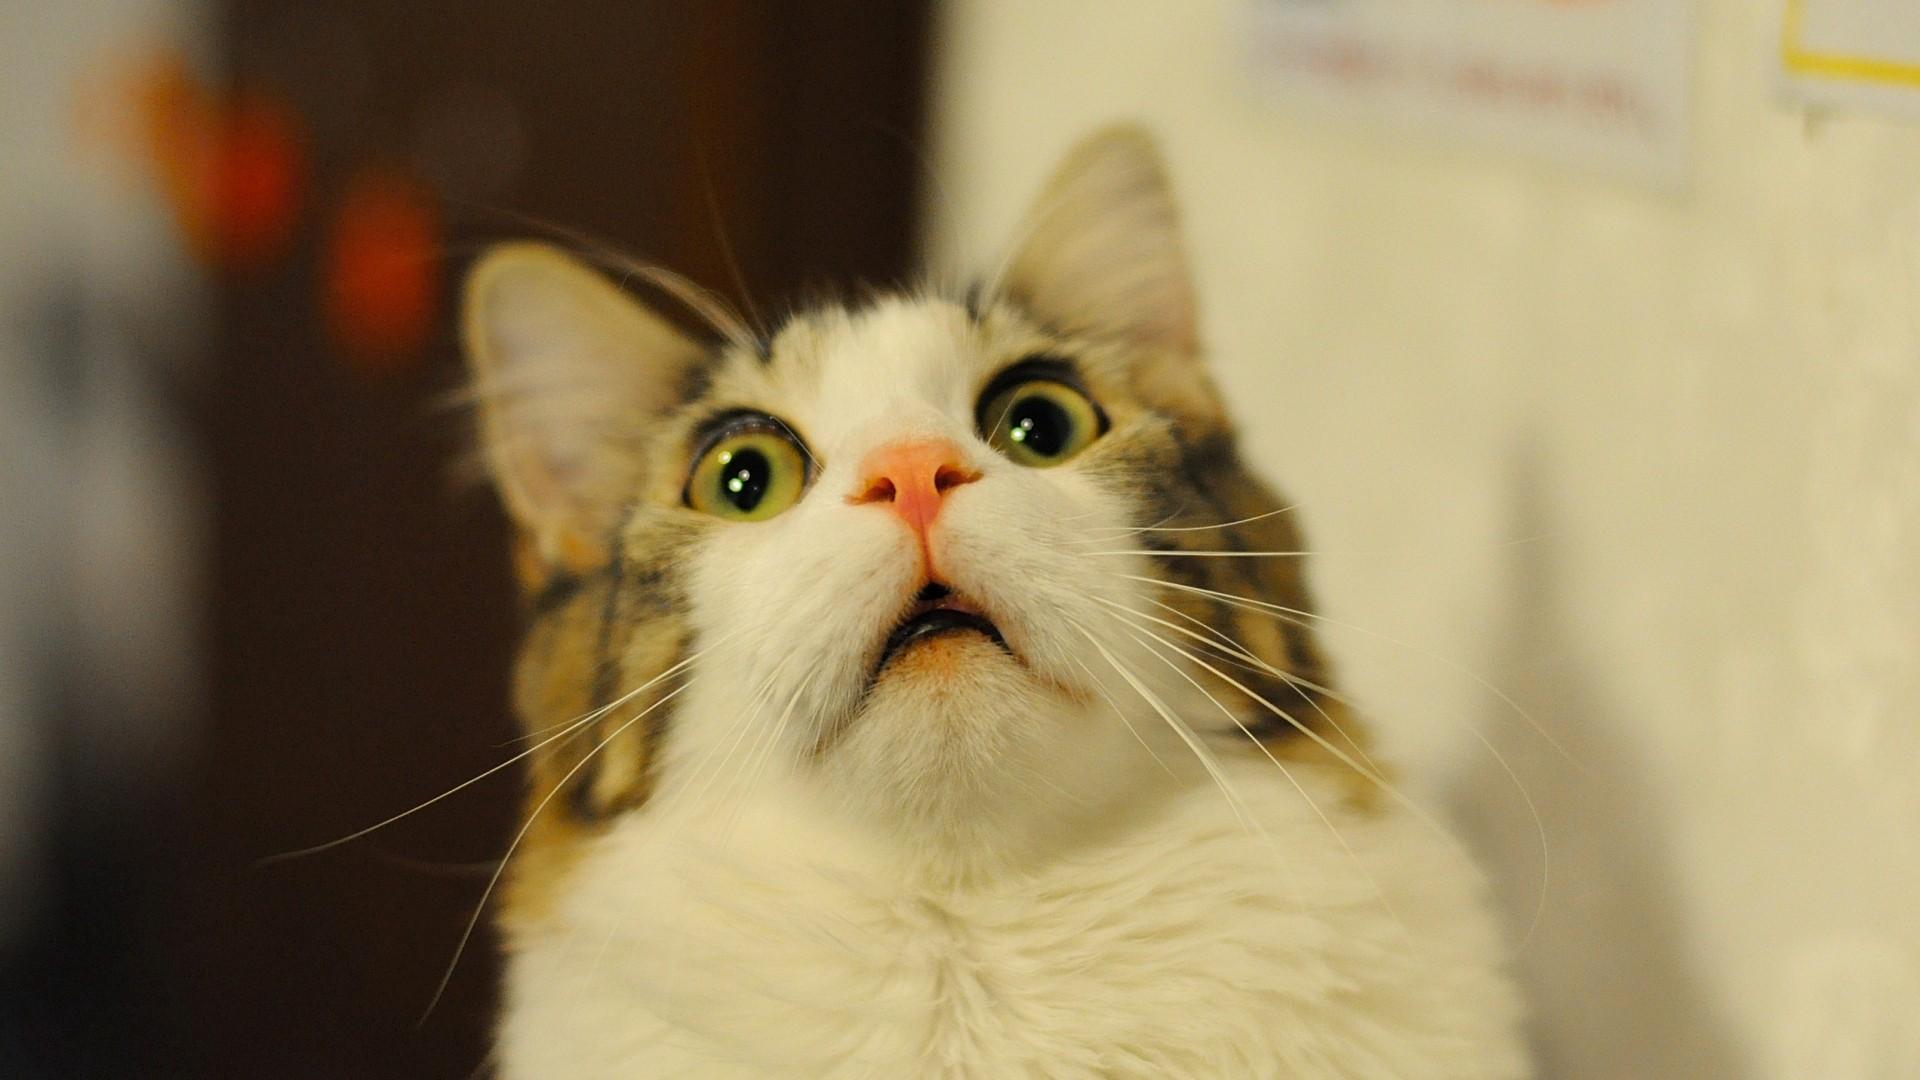
\includegraphics[width=.5\linewidth]{img/cat_surprised}};
            \end{tikzpicture}%
          \end{uncoverenv}%
              \note[item]<.>{
                Nur weil wir die 750 Zeilen pro Minute sein lassen, heißt es nicht das es einfach wird!
              }
              \note[item]<.>{
                Ich werde euch die wichtigsten Elemente präsentieren, die bei der Entwicklung der Makrosprache, bzw. Programmiersprache, durchlaufen wurden.
              }
              \note[item]<.>{
                Dazu zählt auch dieses UML Diagramm, welches eine wichtige Grundlage ist. -- Es sieht schlimmer aus als es ist\ldots
              }
          \action{}
        \end{uncoverenv}
            \note[item]<.>{
              Der \textbf{Invoker} wird von dem \textbf{CommandProvider} an den \textbf{Client} gegeben -- der \textbf{Client} kann z.B ein Knopf in einer GUI sein.
            }
            \note[item]<.>{
              Der \textbf{HistoryStack} sorgt dafür, dass \textbf{Command}s rückgängig gemacht bzw. wiederhergestellt werden können.
            }
            \note[item]<.>{
              Das \textbf{Command} ist die Elternklasse von dem \textbf{ConcreteCommand} welche ihre Funktionalität in der \textbf{execute} Methode implementiert. Die einen Rückgabewert vom Typ any erlaubt.
            }
            \note[item]<.>{
              Ebenso zu beachten ist die \textbf{map<string, any>}. Diese erlaubt es beliebig viele Daten, mit beliebigen Datentypen, typsicher als Parameter zu übergeben -- ohne die Methodensignatur zu verändern.
            }
            \note[item]<.>{
              Der any Typ -- der beliebige Datentypen typsicher wrapped -- wird in C++17 enthalten sein.
            }
    \end{itemize}
  \end{frame}

%---------------------------------
% Anforderungen
%---------------------------------
\section{Anforderungen}
    \note[enumerate]{
      \item Anforderungen an die Lösung\ldots
    }

  \begin{frame}{Anforderungen}
    \begin{itemize}
      \item<+- | alert@+-+(1)>
        Dynamisches Typesystem
            \note[item]<.>{
              Die Makros sollten davon profitieren, dass die Commands Rückgabewerte und Parameter haben. Das heißt, dass es eine Möglichkeit geben muss, dass ``unbekannte'' Datentypen zwischengespeichert werden.
            }
            \note[item]<.>{
              Unbekannt impliziert, dass die Makrosprache mit allen Datentypen arbeiten können muss, nicht nur den primitiven, die als Literals in dem Makro erstellt werden können.
            }
            \note[item]<.>{
              Durch das dynamische Typsystem soll es also möglich sein, so etwas zu schreiben \ldots
            }
        \begin{uncoverenv}<+-+>%
          \tabto{4.6cm}
          \myMIn$var a = 10; a = "10";$
        \end{uncoverenv}
            \note[item]<.>{
              Hier wird der Variable \textbf{a} beim ersten Mal ein Integer zugewiesen und beim zweiten Mal ein String.
            }
            \note[item]<.>{
              Die Lösung für das zwischenspeichern ist der any Typ, der von dem Command-Pattern genutzt wird.
            }
      \item<+- | alert@+-+(1)>
        Kontrollfluss
            \note[item]<.>{
              Die Makros sollten auch eine Möglichkeit haben, auf den Zustand der Anwendung zu reagieren.

              Ein Beispiel wäre \ldots
            }
        \begin{uncoverenv}<+-+>
          \tabto{4.6cm}
          \myMIn$if(has_unsaved()) \{ save(); \}$\hspace*{-4cm} % Fixes unwanted linebreak
        \end{uncoverenv}
            \note[item]<.>{
              Das ein Makro nur probiert zu speichern, wenn es etwas zum speichern gibt.
            }
            \note[item]<.>{
              Generell sollte speichern schnell gehen, allerdings kann es passieren, dass eine mehrere Gigabyte große Datei geschrieben werden muss, was dem Nutzer nicht zumuten ist.
            }
      \item<+- | alert@+-+(2)>
        Benutzerfreundlichkeit
            \note[item]<.>{
              Außerdem soll die Makrosprache für den Benutzer leicht zu verstehen sein. Da der Benutzer auch der Endkunde sein kann \ldots
            }
        \begin{uncoverenv}<+>
          \begin{tikzpicture}[overlay, remember picture]%
            \node[anchor=north] at (page cs:-0.0125,-0.1) (usability exmacro) {
              \begin{myInvBox}[width=.9\linewidth]
                \lstinputlisting[style=MyMacroStyle, backgroundcolor=, numbers=none, frame=,]{img/exmacro.txt}
              \end{myInvBox}
            };%
          \end{tikzpicture}%
        \end{uncoverenv}
            \note[item]<.>{
              Der Syntax sollte also deutlich machen, was passieren wird.
            }
            \note[item]<.>{
              Durch \textbf$def$ wird automatisch klar, das eine Funktion definiert wird und \textbf$var$ definiert eine Variable.
            }
            \note[item]<.>{
              Da die Implementation des CommandPatterns eine Map nutzt, um die Parameter des Commands anzugeben, habe ich mich entschieden named parameter zu nutzen (\textbf{foo:bar}). Diese schreiben keine Reihenfolge vor und ermöglichen das überladen von Funktionen anhand der Parameternamen.
            }
            \note[item]<.>{
              Aber in meine Augen ist Syntax nur ein kleiner Punkt der Benutzerfreundlichkeit \ldots
            }
        \begin{uncoverenv}<+>
         \begin{tikzpicture}[overlay, remember picture]%
            \node[anchor=north] at (page cs:-0.0125,-0.1) (usability error2) {
              \begin{myInvBox}[width=.9\linewidth]
                \lstinputlisting[backgroundcolor=, numbers=none, frame=]{img/error2.txt}
              \end{myInvBox}
            };%
          \end{tikzpicture}%
        \end{uncoverenv}
            \note[item]<.>{
              In dem Beispiel wurde ein Semikolon in der main Methode vergessen, was die beiden Fehlermeldungen schnell deutlich machen.
            }
            \note[item]<.>{
              Wenn der Nutzer einen Fehler macht, soll dieser möglichst einfach zu finden sein -- man will mit einem Tool arbeiten, nicht dagegen kämpfen.
            }
            \note[item]<.>{
              Die Fehlermeldungen müssen dem Nutzer nicht nur sagen was falsch ist, sondern auch wo und weshalb.
            }
        \item<+- | alert@+>
          Wartbarkeit und Macht
              \note[item]<.>{
                Neben der Wartbarkeit, war auch die Macht dieser Makrosprache wichtig.
              }
              \note[item]<.>{
                Wie der Syntax gezeigt hat, geht die Sprache in die Richtung von Scripts, man kann Funktionen anlegen, primitive Datentypen nutzen und hat Kontrollstrukturen zur Verfügung.
              }
              \note[item]<.>{
                Da die Makros letztendlich nur auf Commands arbeiten können, ist das Gefahrenpotenzial -- was von unwissenden Nutzern ausgeht -- größtenteils eingeschränkt.
              }
    \end{itemize}
  \end{frame}

%---------------------------------
% Konzeption
%---------------------------------
\section{Konzeption}
    \note[enumerate]{
      \item Kommen wir nun zur Konzeption
      \item Die folgende Liste zeigt nicht nur, was entwickelt werden musste, sondern auch den abstrakten Ablauf, der beim Ausführen eines Makros stattfindet.
    }

  %---------------------------------
  % Was wurde entwickelt?
  %---------------------------------
  \begin{frame}{Was wurde entwickelt?}
    \begin{itemize}[<+- | alert@+>]
      \item<+- | alert@+-+(1)>
        Tokenizer
            \note[item]<.>{
              Als erstes brauchen wir einen Tokenizer.
            }
            \note[item]<.>{
              Der Tokenizer muss den String / das Makro zu einer Liste von Tokens -- also Teilstücke -- verwandeln \ldots
            }
        \begin{uncoverenv}<+-+>%
          \begin{tikzpicture}[overlay, remember picture, railroad]%
            \node[anchor=west, yshift=-.9em] at (page cs:-.4,0) (tokenizerMacro) {%
              \begin{myInvBox}[width=.36\linewidth]%
                \lstinputlisting[style=MyMacroStyle, backgroundcolor=, numbers=none, frame=,]{img/exmacro_2.txt}%
              \end{myInvBox}%
            };%
            \node[right=1of tokenizerMacro] (tokenizerTokens) {%
              \begin{myInvBox}[width=.9\linewidth]%
                \lstinputlisting[backgroundcolor=, numbers=none, frame=,]{img/exmacro_2_tok.txt}%
              \end{myInvBox}%
            };%
            \graph[railroad]{(tokenizerMacro)->(tokenizerTokens);};%
          \end{tikzpicture}%
        \end{uncoverenv}%
            \note[item]<.>{
              Wichtig ist, dass bei dem erstellen der Liste, keine nützlichen Informationen verloren gehen.
            }
            \note[item]<.>{
              Zwar wird die Reihenfolge durch das Tokenizen nicht verändert, allerdings gehen überflüssige Leerzeichen und Zeilenumbrüche verloren.
            }
            \note[item]<.>{
              Diese sind für Fehlermeldungen extrem wichtig und müssen mitgespeichert werden.
            }

      \item
        \temporal<.>{}{Abstrakter Syntaxbaum}{AST}
            \note[item]<.>{
              Für den Folgenden Schritt muss es Klassen geben, die einen abstrakten Syntaxbaum bilden.
            }
            \note[item]<.>{
              Ein Abstrakter Syntaxbaum beschreibt den Syntax aus dem Makro, ohne Informationsverlust und ist nur ein passiver Bestandteil des Ablaufes.
            }
            \note[item]<.>{
              ASTs werden genutzt, da es einfacher ist mit ihnen als Datenstruktur zu arbeiten, als mit einem String.
            }
            \note[item]<.>{
              Die meisten Elemente des Syntaxes lassen sich als Klasseninstanzen in dem AST wiederfinden. Prominente Ausnahmen sind Klammern, Semikolons und Leerzeichen.
            }
      \item<+- | alert@+-+(1)>
        Parser\tikzmark{parser}{}%
            \note[item]<.>{
              Das nächste aktive Element ist ein Parser.
            }
            \note[item]<.>{
              Der Parser ist dafür zuständig, dass die Liste von Tokens in einen abstrakten Syntaxbaum umgewandelt werden.
              \ldots
            }%
        \begin{uncoverenv}<+-+>%
          \begin{tikzpicture}[overlay, remember picture, railroad]%
            \node[anchor=west, yshift=-.6em] at (page cs:-.4,0) (parserMacro) {%
              \begin{myInvBox}[width=.28\linewidth]%
                \lstinputlisting[backgroundcolor=, numbers=none, frame=,]{img/exmacro_2_tok.txt}%
              \end{myInvBox}%
            };%
            \node[right=.5of parserMacro] (parserTokens) {%
              \begin{myInvBox}[width=.9\linewidth]%
                \lstinputlisting[backgroundcolor=, numbers=none, frame=,]{img/exmacro_2_ast.txt}%
              \end{myInvBox}%
            };%
            \graph[railroad]{(parserMacro)->($(parserTokens.west)+(0:.6)$);};%
            \end{tikzpicture}%
        \end{uncoverenv}%
            \note[item]<.>{
              Das heißt das der Parser die Tokens in \textbf{diese} Form überführen muss.
            }%
            \note[item]<.>{
              Die \textbf{@-Symbole} weisen auf eine AST Objektinstanz hin.
            }%
            \note[item]<.>{
              Das was in den Klammern (\textbf{\{\}}) eingeschlossen ist, ist ein Bestandteil des umschließenden Objektes.
            }%
      \item<+- | alert@+-+(1)>
        Analyser\tikzmark{analyser}{}%
            \note[item]<.>{
              Als vorletztes Element bedarf es einem Analyser.
            }
            \note[item]<.>{
              Der Analyser ist dafür da, um Fehler zu finden, die nicht aus dem Parsen hervorgehen. Also Fehler die nicht syntaktisch sind, oder nur schwer beim Parsen zu finden sind.
              \ldots
            }
        \begin{uncoverenv}<+-+>%
          \begin{tikzpicture}[overlay, remember picture]%
            \node[coordinate] at (page cs:-.4,0) (analyserMacroHelper){};
            \node[anchor=north west, yshift=.6em] at (analyserMacroHelper |- analyser) (analyserMacro) {%
              \myMIn$def gun()\{ break; \}$
            };%
          \end{tikzpicture}%
        \end{uncoverenv}
            \note[item]<.>{
              Ein Beispiel wäre die Funktion \textbf{gun}.
              }
            \note[item]<.>{
              Der AST kann den Code darstellen. Eine Funktionsdefinition, die in dem Funktionsscope ein break Element hat.
            }
            \note[item]<.>{
              Bloß macht dies wenig Sinn, da \textbf{break} nur in Schleifen eine Funktion hat.
            }
            \note[item]<.>{
              Es ist also wichtig dem Nutzer zu sagen, dass das was er geschrieben hat höchst wahrscheinlich nicht das ist, was er erwartet.
            }
      \item
        Interpreter
            \note[item]<.>{
              Letztlich bedarf es einem Interpreter.
            }
            \note[item]<.>{
              Der Interpreter interpretiert den AST, den der Parser erzeugt hat und ist die Komponente -- bzw. der Client, aus dem CommandPattern -- der die Commands ausführt.
            }
            \note[item]<.>{
              Somit kommen wir zu wir \ldots (zu weiteren UML Diagrammen)
            }
    \end{itemize}
  \end{frame}

  %---------------------------------
  % AST Klassenhierarchie
  %---------------------------------
  \begin{frame}{AST Klassenhierarchie}
    \begin{uncoverenv}<+>%
      \begin{tikzpicture}[overlay, remember picture]%
        \node[anchor=center] at (page cs:0,0) (commanduml-cat_surprised) {
\includegraphics[width=.6\linewidth]{img/grumpy_cat}};
      \end{tikzpicture}%
    \end{uncoverenv}%
        \note[item]<.>{
          Zu weiteren UML Diagrammen.
        }
        \note[item]<.>{
          Für meinen Geschmack helfen die Diagramme nicht genug.
        }
        \note[item]<.>{
          Sie sind aber die beste Möglichkeit, die ich kenne, anderen Menschen mein Wissen, über die Datenstrukturen, zu mitzuteilen.
        }

    \begin{actionenv}<+->
      \begin{tikzpicture}[remember picture,overlay,every node/.style={anchor=center}]%
        \node at(current page.center) (ASTuml) {%
          \scalebox{.9}{%
            \myInput{img/ASTuml.tikz}%
          }
        };
      \end{tikzpicture}%
          \note[item]<.>{
            Die AST Klassenhierarchie.
          }
          \note[item]<.>{
            Alle abstrakten Syntax Klassen haben die \textbf{AST} Klasse als Elternklasse. Diese hat ein \textbf{Token}, welches das Stück des Makros enthält, welches es repräsentieren soll.
          }
    \end{actionenv}
  \end{frame}

  \begin{frame}{AST Scope}
    \begin{tikzpicture}[remember picture,overlay,every node/.style={anchor=center}]%
      \node at(current page.center) (Scopeuml) {%
        \scalebox{.7}{%
          \myInput{img/Scopeuml.tikz}%
        }
      };
    \end{tikzpicture}%
        \note[item]{
          Das \textbf{Scope} kann Instanzen von allen AST Klassen aufnehmen.
        }
        \note[item]{
          Durch die Aufnahme von anderen AST Instanzen wird hier ein Teil des Baumes erstellt.
        }
  \end{frame}

  \begin{frame}{AST Klassen}
    \begin{tikzpicture}[remember picture,overlay,every node/.style={anchor=center}]%
      \node at(current page.center) (Conditionuml) {%
        \scalebox{.7}{%
          \myInput{img/Conditionuml.tikz}%
        }
      };
    \end{tikzpicture}%
        \note[item]{
          Dieses UML Diagramm zeigt die restlichen Abhängigkeiten der AST Klassen -- die meisten Verbindungen sollten Selbstverständlich sein.
        }
        \note[item]{
          Ein Bestandteil einer \textbf{Funktion} ist ein \textbf{Scope}. Ein \textbf{Loop} besteht aus einem \textbf{Scope} und einer \textbf{Condition}. Eine \textbf{Condition} kann aus \textbf{Variablen}, Funktionsaufrufen (\textbf{Callable}) usw. bestehen.
        }
  \end{frame}

  \begin{frame}{Parser Klassen}
    \begin{tikzpicture}[remember picture,overlay,every node/.style={anchor=center}]%
      \node at(current page.center) (parserpackuml) {%
        \scalebox{.7}{%
          \myInput{img/parserpackuml.tikz}%
        }
      };
    \end{tikzpicture}%
        \note[item]{
          Das vorletzte Diagramm zeigt die Parser Klassen.
        }
        \note[item]{
          Der \textbf{Parser} nutzt den \textbf{Tokenizer} um eine \textbf{TokenList} von dem Makrostring zu erstellen.
        }
        \note[item]{
          Diese TokenListe wandelt er dann in einen \textbf{AST} um.
        }
        \note[item]{
          Der produzierte AST wird dann von dem \textbf{Analyser} überprüft.
        }
  \end{frame}

  \begin{frame}{Interpreter Klassen}
    \begin{uncoverenv}<+-+(1)>%
      \begin{tikzpicture}[remember picture,overlay,every node/.style={anchor=center}]%
        \node at(current page.center) (interpreterpackuml) {%
            \myInput{img/interpreterpackuml.tikz}%
        };
      \end{tikzpicture}%
          \note[item]<.>{
            Letztlich die Interpreter Klassen.
          }
          \note[item]<.>{
            Der \textbf{Interpreter} nutzt den \textbf{Parser} um einen AST zu erzeugen, den er dann interpretieren kann.
          }
          \note[item]<.>{
            Um dies zu tun, muss der Interpreter auch Daten verwalten. Das wird von dem \textbf{Stack} übernommen.
          }
          \note[item]<.>{
            Der Stack bildet einen Stack mit Instanzen von sich selber \ldots
          }
      \begin{uncoverenv}<+>%
        \begin{tikzpicture}[overlay, remember picture]%
          \node[anchor=center] at (page cs:-.5,-.4) (commanduml-no_you_didnt_cat) {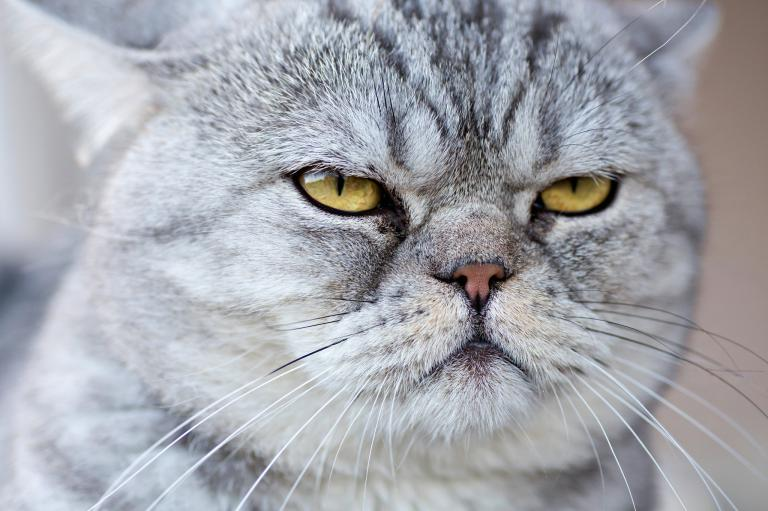
\includegraphics[width=.5\linewidth]{img/no_you_didnt_cat}};
        \end{tikzpicture}%
      \end{uncoverenv}%
          \note[item]<.>{
             Diese Art und Weise einen Stack aufzubauen ist normal in C oder C++, da man dort Pointer zur Verfügung hat.
          }
    \end{uncoverenv}
    \begin{uncoverenv}<+-+>%
      \begin{tikzpicture}[remember picture,overlay,every node/.style={anchor=center}]%
        \node at(current page.center) (stackex) {%
            \myInput{img/stackex.tikz}%
        };
      \end{tikzpicture}%
          \note[item]<.>{
            \textbf{Hier} wird der Stack durch die drei Stack Instanzen (\textbf{0, 1 und 2}) gebildet.
          }
          \note[item]<.>{
            Ein späteres Beispiel wird wahrscheinlich mehr Aufschluss über die Funktionsweise und Vorteile bringen.
          }
    \end{uncoverenv}
    \begin{uncoverenv}<+-+>%
      \begin{tikzpicture}[remember picture,overlay,every node/.style={anchor=center}]%
        \node at(current page.center) (interpreterpackuml) {%
            \myInput{img/interpreterpackuml.tikz}%
        };
      \end{tikzpicture}%
          \note[item]<.>{
            Der \textbf{OperatorProvider} wird von dem Interpreter genutzt um die \textbf{Operator}en -- wie $+$ und $-$ -- auf Variablen anzuwenden.
          }
          \note[item]<.>{
            Die Nutzung eines OperatorProviders sorgt dafür, dass Operatoren für beliebige Datentypen angeboten werden können, ohne den Interpreter anzupassen.
          }
          \note[item]<.>{
            Der Code des OperatorProviders ist sehr Interessant -- leider haben wir nicht genug Zeit um diesen durchzugehen. Weshalb ich euch wieder mit dem any Typ abspeisen muss, der auch hier ein wichtiger Eckpunkt ist.
          }
          \note[item]<.>{
            Um Funktionsaufrufe auszuführen -- die nicht zu selber definierten Funktionen aus dem Makro führen -- nutzt der Interpreter den \textbf{CommandProvider}, die letztendlich die Komponente sind, die die Anwendung verändern.
          }
    \end{uncoverenv}
  \end{frame}

%---------------------------------
% Realisierung
%---------------------------------
\section{Realisierung}
    \note[enumerate]{
      \item Das war die trockene Theorie.
      \item In den folgenden Folien werde ich an dem vorherigen Beispiel die einzelnen Schritte erklären, die beim Interpretieren durchlaufen werden. Also das, was in der Demo im Hintergrund passieren wird.
    }

  %---------------------------------
  % Tokenizer
  %---------------------------------
  \begin{frame}{Tokenizer}
    \pause
        \note[item]<.>{
          Der Tokenizer hat drei Hauptartenarten von Tokens
        }
    \begin{itemize}[<+- | alert@+>]
      \item
        Normale Tokens
            \note[item]<.>{
              Normale Tokens werden durch alle Zeichen getrennt, die keine Buchstaben, Zahlen oder Unterstriche sind.
            }
            \note[item]<.>{
               Oder durch sich selber ein Token bilden  z.B. eine Klammer.
            }

      \item<+- | alert@+-+(1)>
        Strings\tikzmark{TokenizerString}{}
            \note[item]<.>{
              Strings sind besonders, \ldots (da sie ein Token bilden müssen)
            }
        \begin{uncoverenv}<+-+>%
          \begin{tikzpicture}[overlay, remember picture]%
            \node[coordinate] at (page cs:-.2,0) (TokenizerStringHelper){};
            \node[anchor=north west, yshift=.6em] at (TokenizerStringHelper |- TokenizerString) (TokenizerStringCode) {%
              \myMIn$print("print(\\"Hallo Welt!\\"")$
            };%
          \end{tikzpicture}%
        \end{uncoverenv}
            \note[item]<.>{
              Da sie ein Token bilden müssen. Sonst würden die Leerzeichen verloren gehen.
            }
            \note[item]<.>{
              Außerdem müssen die Anführungszeichen richtig interpretiert werden.
            }

      \item<+- | alert@+-+(1)>
        Floats\tikzmark{TokenizerFloat}{}
            \note[item]<.>{
              Dezimalzahlen sind -- ähnlich wie Strings -- besondere Tokens\ldots (Da die beiden Teile der Zahl durch ein Punkt getrennt werden.)
            }


        \begin{uncoverenv}<+-+>%
          \begin{tikzpicture}[overlay, remember picture]%
            \node[coordinate] at (page cs:-.2,0) (TokenizerFloatHelper){};
            \node[anchor=north west, yshift=.6em] at (TokenizerFloatHelper |- TokenizerFloat) (TokenizerFloatCode) {%
              \myMinin{0.1} oder \myMinin{.1234}
            };%
          \end{tikzpicture}%
        \end{uncoverenv}
            \note[item]<.>{
              Da die beiden Teile der Zahl durch ein Punkt getrennt werden.
            }
    \end{itemize}
  \end{frame}

  %---------------------------------
  % Parser
  %---------------------------------
  \begin{frame}{Parser}
    \pause
        \note[item]<.>{
          Kommen wir zu den Parser.
        }
        \note[item]<.>{
          Der Parser ist der komplexeste Teil der Arbeit -- aus Zeitgründen werde ich nur zwei wichtige Punkte anschneiden und ansonsten behaupten, das es einfach funktioniert.
        }
    \begin{itemize}[<+- | alert@+>]
      \item
        Recursive descent
            \note[item]<.>{
              Der Parser wurde recursive descent implementiert.
            }
            \note[item]<.>{
              Das heißt, dass die Grammatik der Sprache durch Funktionsaufrufe abgebildet wird. Anstelle von Zustandsübergangstabellen.
            }
            \note[item]<.>{
              Was das bedeutet, zeige ich an dem folgenden Punkt.
            }
      \item<+- | alert@+-+(2)>
        Operatoren\tikzmark{ParserOperator}{}
            \note[item]<.>{
              Ein schwieriger Punkt beim parsen ist das zusammenstellen der Operatoren\ldots
            }

          \begin{uncoverenv}<+-+>%
            \begin{tikzpicture}[overlay, remember picture]%
              \node[coordinate] at (page cs:-.2,0) (ParserOperatorHelper){};
              \node[anchor=north west, yshift=.6em] at (ParserOperatorHelper |- ParserOperator) (ParserOperatorCode) {%
                \myMIn$var foo = 1 - 1;$



                % FIXME each step with line to symbolise scope!!!!



              };%
            \end{tikzpicture}%
          \end{uncoverenv}
            \note[item]<.>{
              Der Ablauf wäre wie folgt:
            }
            \note[item]<.>{
              Parsen einer Variablen Deklaration(\textbf{var}). In dieser Funktion wird die Funktion zum Wertzuweisung -- bzw. Operator -- parsen(\textbf{=}) aufgerufen. Welche dann die Funktion zum parsen eines Literals(\textbf{1}) aufruft. Diese returned zurück zur Zuweisungsfunktion, die dann die Funktion zum parsen von Operatoren(\textbf{-}) aufruft. Welche wiederum ein die Funktion für Literals(\textbf{1}) aufruft.
            }
            \note[item]<.>{
              Durch diese Reihenfolge wird allerdings kein Baum erzeugt, sondern eine Liste. Von Literal operator Literal.
            }
            \note[item]<.>{
              Die Liste muss durch einen zweiten Schritt in der Operator Funktion dann zu einem Operator mit zwei Literals umgewandelt werden.
            }

          \begin{uncoverenv}<+-+>%
            \begin{tikzpicture}[overlay, remember picture]%
              \node[coordinate] at (page cs:-.2,0) (ParserOperatorHelper){};
              \node[anchor=north west, yshift=.6em] at (ParserOperatorHelper |- ParserOperator) (ParserOperatorCode) {%
                \myMIn$var foo = 1 --- 1;$
              };%
            \end{tikzpicture}%
          \end{uncoverenv}
            \note[item]<.>{
              Und hier?
            }
            \note[item]<.>{
              Hier wird das zweite Literal zweimal negiert und dann vom ersten abgezogen.
            }
            \note[item]<.>{
              Wie genau das Abläuft kann ich leider aus Zeitgründen nicht zeigen.
            }
    \end{itemize}
  \end{frame}

  %---------------------------------
  % Parser
  %---------------------------------
  \begin{frame}{Interpreter}
    \pause
        \note[item]<.>{
          Womit wir beim Interpreter wären.
        }
        \note[item]<.>{
          Der Interpreter ist sehr einfach -- um nicht primitiv zu sagen -- wodurch er wenig Logik besitzt, die zu erklären ist.
        }
    \begin{itemize}[<+- | alert@+>]
      \item Läuft den AST ab
          \note[item]<.>{
            Der Interpreter läuft den generierten AST ab.
          }
      \item \myMin{OperatorProvider}
          \note[item]<.>{
            Macht sich den OperatorProvider für Operationen zunutze
          }
      \item \myMin{CommandProvider}
          \note[item]<.>{
            Ruft Commands über den CommandProvider auf
          }
      \item \myMin{Stack}
          \note[item]<.>{
            Und überlässt die Daten und Funktionsverwaltung dem Stack.
          }
    \end{itemize}
  \end{frame}


  \begin{frame}{Interpreter/Stack}
    \pause
        \note[item]<.>{
          Somit kommen wir zum Letzten Teil -- dem Stack bzw. was beim interpretieren passiert.
        }
    \begin{uncoverenv}<+>%
      \begin{tikzpicture}[overlay, remember picture]%
        \node[anchor=center] at (page cs:.5,0) (stack int) {\myInput{img/int1.tikz}};
        \node[anchor=center] at (page cs:-.5,0) (stack code) {\lstinputlisting[style=MyMacroStyle, backgroundcolor=, numbers=none, frame=,escapechar=°]{img/int_macro.txt}};
        \node[anchor=center,red,fill,circle,inner sep=.3ex] (at_pos) at ($(int_macro_l_0)-(0:.4)$){};
      \end{tikzpicture}%
    \end{uncoverenv}%
        \note[item]<.>{
          Der rote Punkt gibt die Zeile an, welche gerade interpretiert wird bzw. den Stack verändert.
        }
        \note[item]<.>{
          Am Anfang gibt es eine Root Node, die durch die root Stack Instanz abgebildet wird\ldots
        }

    \begin{uncoverenv}<+>%
      \begin{tikzpicture}[overlay, remember picture]%
        \node[anchor=center] at (page cs:.5,0) (stack int) {\myInput{img/int2.tikz}};
        \node[anchor=center] at (page cs:-.5,0) (stack code) {\lstinputlisting[style=MyMacroStyle, backgroundcolor=, numbers=none, frame=,escapechar=°]{img/int_macro.txt}};
        \node[anchor=center,red,fill,circle,inner sep=.3ex] (at_pos) at ($(int_macro_l_1)-(0:.4)$){};
      \end{tikzpicture}%
    \end{uncoverenv}%
        \note[item]<.>{
          Als ersten Schritt definiert der Interpreter die Funktionen eines Scopes, bevor er anfängt diese zu interpretieren.
        }
        \note[item]<.>{
          Dadurch kann \textbf{main}\ldots( vor \textbf{foo} definiert werden.)
        }

    \begin{uncoverenv}<+>%
      \begin{tikzpicture}[overlay, remember picture]%
        \node[anchor=center] at (page cs:.5,0) (stack int) {\myInput{img/int3.tikz}};
        \node[anchor=center] at (page cs:-.5,0) (stack code) {\lstinputlisting[style=MyMacroStyle, backgroundcolor=, numbers=none, frame=,escapechar=°]{img/int_macro.txt}};
        \node[anchor=center,red,fill,circle,inner sep=.3ex] (at_pos) at ($(int_macro_l_7)-(0:.4)$){};
      \end{tikzpicture}%
    \end{uncoverenv}%
        \note[item]<.>{
         Vor \textbf{foo} definiert werden.
        }

    \begin{uncoverenv}<+>%
      \begin{tikzpicture}[overlay, remember picture]%
        \node[anchor=center] at (page cs:.5,0) (stack int) {\myInput{img/int5.tikz}};
        \node[anchor=center] at (page cs:-.5,0) (stack code) {\lstinputlisting[style=MyMacroStyle, backgroundcolor=, numbers=none, frame=,escapechar=°]{img/int_macro.txt}};
        \node[anchor=center,red,fill,circle,inner sep=.3ex] (at_pos) at ($(int_macro_l_2)-(0:.4)$){};
      \end{tikzpicture}%
    \end{uncoverenv}%
        \note[item]<.>{
          Als nächstes wird die \textbf{main} Methode aufgerufen.
        }
        \note[item]<.>{
          Dadurch wird eine neue Stack Instanz erzeugt, in der eine Variable \textbf{bar} angelegt wird.\ldots
        }

    \begin{uncoverenv}<+>%
      \begin{tikzpicture}[overlay, remember picture]%
        \node[anchor=center] at (page cs:.5,0) (stack int) {\myInput{img/int6.tikz}};
        \node[anchor=center] at (page cs:-.5,0) (stack code) {\lstinputlisting[style=MyMacroStyle, backgroundcolor=, numbers=none, frame=,escapechar=°]{img/int_macro.txt}};
        \node[anchor=center,red,fill,circle,inner sep=.3ex] (at_pos) at ($(int_macro_l_2)-(0:.4)$){};
      \end{tikzpicture}%
    \end{uncoverenv}%
        \note[item]<.>{
          Der String ``Eins Leerzeichen'' wird bar zugewiesen.
        }

    \begin{uncoverenv}<+>%
      \begin{tikzpicture}[overlay, remember picture]%
        \node[anchor=center] at (page cs:.5,0) (stack int) {\myInput{img/int8.tikz}};
        \node[anchor=center] at (page cs:-.5,0) (stack code) {\lstinputlisting[style=MyMacroStyle, backgroundcolor=, numbers=none, frame=,escapechar=°]{img/int_macro.txt}};
        \node[anchor=center,red,fill,circle,inner sep=.3ex] (at_pos) at ($(int_macro_l_4)-(0:.4)$){};
      \end{tikzpicture}%
    \end{uncoverenv}%
        \note[item]<.>{
          Danach wird \textbf{fun} aufgerufen, wodurch wieder eine Stack Instanz (\textbf{fun}) zu dem Stack hinzugefügt wird.
        }
        \note[item]<.>{
          Der Stackinstanz wird \textbf{foo} als Alias auf \textbf{bar} mitgegeben.
        }


    \begin{uncoverenv}<+>%
      \begin{tikzpicture}[overlay, remember picture]%
        \node[anchor=center] at (page cs:.4,0) (stack int) {\myInput{img/intstack.tikz}};
        \node[anchor=center] at (page cs:-.5,0) (stack code) {\lstinputlisting[style=MyMacroStyle, backgroundcolor=, numbers=none, frame=,escapechar=°]{img/int_macro.txt}};
        \node[anchor=center,red,fill,circle,inner sep=.3ex] (at_pos) at ($(int_macro_l_4)-(0:.4)$){};
      \end{tikzpicture}%
    \end{uncoverenv}%
        \note[item]<.>{
          Es gibt nun also zwei Stacks die jeweils aus zwei Stack Instanzen bestehen -- bzw. im nächsten Schritt aus zwei und drei.
        }
        \note[item]<.>{
          Wieso?
        }
        \note[item]<.>{
          Wenn es nur einen Stack geben würde -- der \textbf{fun Stack} also den \textbf{main Stack} haben würde, könnte man aus der fun Funktion die bar Variable verändern. Das will man aber nicht.
        }

    \begin{uncoverenv}<+>%
      \begin{tikzpicture}[overlay, remember picture]%
        \node[anchor=center] at (page cs:.5,0) (stack int) {\myInput{img/int9.tikz}};
        \node[anchor=center] at (page cs:-.5,0) (stack code) {\lstinputlisting[style=MyMacroStyle, backgroundcolor=, numbers=none, frame=,escapechar=°]{img/int_macro.txt}};
        \node[anchor=center,red,fill,circle,inner sep=.3ex] (at_pos) at ($(int_macro_l_9)-(0:.4)$){};
      \end{tikzpicture}%
    \end{uncoverenv}%
        \note[item]<.>{
          Bei dem referenzieren von foo -- also bar -- ist nur lesen erlaubt.
        }
        \note[item]<.>{
          Das heißt nach dem Addieren von dem String ``Eins Leerzeichen'' und der Dezimalzahl ``1.1'', wird der Alias gelöscht und eine Variable foo angelegt, die das Ergebnis speichert wird.
        }
        \note[item]<.>{
          Abgesehen von Scope Sicherheit bietet dieses Verfahren weniger Speicherverbrauch und sollte deswegen generell schneller sein.
        }

    \begin{uncoverenv}<+-+(1)>%
      \begin{tikzpicture}[overlay, remember picture]%
        \node[anchor=center] at (page cs:.5,0) (stack int) {\myInput{img/int10.tikz}};
        \node[anchor=center] at (page cs:-.5,0) (stack code) {\lstinputlisting[style=MyMacroStyle, backgroundcolor=, numbers=none, frame=,escapechar=°]{img/int_macro.txt}};
        \node[anchor=center,red,fill,circle,inner sep=.3ex] (at_pos) at ($(int_macro_l_4)-(0:.4)$){};
      \end{tikzpicture}%
    \end{uncoverenv}%
        \note[item]<.>{
          Nach dem return aus fun, ist als bar unverändert.
        }
        \note[item]<.>{
          Und der String aus fun wird in die C++ Ebene returned.
        }

    \begin{uncoverenv}<+>%
      \begin{tikzpicture}[overlay, remember picture]%
        \node[anchor=center] at (page cs:0,0) (finish-sleepy) {
\includegraphics[width=.5\linewidth]{img/sleepy_cat}};
      \end{tikzpicture}%
    \end{uncoverenv}%
        \note[item]<.>{
          Ihr habt es geschafft!
        }
        \note[item]<.>{
          Welche Fragen wollt ihr nun schon stellen, bevor ich die kurze Demo zeige?
        }
  \end{frame}

%---------------------------------
% Fragen
%---------------------------------
  \begin{frame}[standout]
    Fragen?
  \end{frame}
      \note[itemize]{
        \item \textbf{Katzen:} Ich habe genug theoretische und zum teil langweilige Präsentationen in meinem Studium gesehen. Dem Trend wollte ich nicht folgen -- und auch wenn meine Präsentation nicht so viel Wissen vermittelt hat, hatte sie zumindest Katzen. Wer reine Theorie will, ist mit meiner THesis besser beraten als mit mir.
      }

%---------------------------------
% Demo
%---------------------------------
  \section{Demo}

%---------------------------------
% Weitere Fragen
%---------------------------------
  \begin{frame}[standout]
    Weitere Fragen?
  \end{frame}
      \note[itemize]{
        \item \textbf{Katzen:} Ich habe genug theoretische und zum teil langweilige Präsentationen in meinem Studium gesehen. Dem Trend wollte ich nicht folgen -- und auch wenn meine Präsentation nicht so viel Wissen vermittelt hat, hatte sie zumindest Katzen. Wer reine Theorie will, ist mit meiner THesis besser beraten als mit mir.
      }

\end{document}

